\documentclass[10pt]{beamer}
\usetheme[
%%% options passed to the outer theme
%    hidetitle,           % hide the (short) title in the sidebar
%    hideauthor,          % hide the (short) author in the sidebar
%    hideinstitute,       % hide the (short) institute in the bottom of the sidebar
%    shownavsym,          % show the navigation symbols
%    width=2cm,           % width of the sidebar (default is 2 cm)
%    hideothersubsections,% hide all subsections but the subsections in the current section
%    hideallsubsections,  % hide all subsections
    left               % right of left position of sidebar (default is right)
%%% options passed to the color theme
%    lightheaderbg,       % use a light header background
  ]{AAUsidebar}

% If you want to change the colors of the various elements in the theme, edit and uncomment the following lines
% Change the bar and sidebar colors:
%\setbeamercolor{AAUsidebar}{fg=red!20,bg=red}
%\setbeamercolor{sidebar}{bg=red!20}
% Change the color of the structural elements:
%\setbeamercolor{structure}{fg=red}
% Change the frame title text color:
%\setbeamercolor{frametitle}{fg=blue}
% Change the normal text color background:
%\setbeamercolor{normal text}{bg=gray!10}
% ... and you can of course change a lot more - see the beamer user manual.


\usepackage[utf8]{inputenc}
\usepackage[english]{babel}
\usepackage[T1]{fontenc}
% Or whatever. Note that the encoding and the font should match. If T1
% does not look nice, try deleting the line with the fontenc.
\usepackage{helvet}

\usepackage{listings} % Required for inserting code snippets

%Changing lis name from 'Listing' to 'Code Example'
\renewcommand{\lstlistingname}{Code Example}

%Defining colors used in our style
\definecolor{color1}{RGB}{0,0,90} % Color of the article title and sections
\definecolor{color2}{RGB}{0,20,20} % Color of the boxes behind the abstract and headings
\definecolor{color3}{RGB}{230, 231, 231} % background
\definecolor{Blue}{RGB}{0, 51, 204} % keywords
\definecolor{Gray}{RGB}{153, 153, 153} % line numbers
\definecolor{PineGlade}{RGB}{204, 204, 153}

%Our style for python
\lstdefinestyle{Python1}{ 
language=Python,
frame=single,
basicstyle=\scriptsize\ttfamily,
backgroundcolor=\color{color3},
keywordstyle=\color{color1}\bf,
captionpos=b,
breakatwhitespace=false,
breaklines=true,
numbers=left, % Location of line numbers, can take the values of: none, left, right
numbersep=6pt, % Distance of line numbers from the code box
numberstyle=\tiny, % Style used for line numbers \color{Gray}
commentstyle=\usefont{T1}{pcr}{m}{sl}\color{color1}
} 

%Our style for SQL
\lstdefinestyle{SQL1}{ 
language=SQL,
frame=single,
basicstyle=\scriptsize\ttfamily,
backgroundcolor=\color{color3},
keywordstyle=\color{color1}\bf,
captionpos=b,
breakatwhitespace=false,
breaklines=true,
numbers=left, % Location of line numbers, can take the values of: none, left, right
numbersep=6pt, % Distance of line numbers from the code box
numberstyle=\tiny, % Style used for line numbers \color{Gray}
commentstyle=\usefont{T1}{pcr}{m}{sl}\color{color1}
} 

\newcommand{\insertcodefile}[2]{\begin{itemize}\item[]\lstinputlisting[caption=#2,label=#1,style=Python1,belowskip=-0.8\baselineskip]{code/#1}\end{itemize}} % The first argument is the script location/filename and the second is a caption for the code

\newcommand{\insertcodefileSQL}[2]{\begin{itemize}\item[]\lstinputlisting[caption=#2,label=#1,style=SQL1,belowskip=-0.8\baselineskip]{code/#1}\end{itemize}} 

\newcommand{\insertcodefileline}[4]{\begin{itemize}\item[]\lstinputlisting[firstnumber=#3,firstline=#3,lastline=#4,caption=#2,label=#1,style=Python1]{code/#1}\end{itemize}}


% colored hyperlinks
\newcommand{\chref}[2]{%
  \href{#1}{{\usebeamercolor[bg]{AAUsidebar}#2}}%
}

\title[Optimizing Modular Factory Configurations]% optional, use only with long paper titles
{Optimizing Modular Factory Configurations}

\subtitle{}  % could also be a conference name

\date{\today}

\author[Alexander Brandborg, Mathias Claus Jensen] % optional, use only with lots of authors
{
	Alexander Brandborg \href{abran13@student.aau.dk}{{\tt abran13@student.aau.dk}}\\
	Mathias Claus Jensen \href{mcje13@student.aau.dk}{{\tt mcje13@student.aau.dk}}\\
}
% - Give the names in the same order as they appear in the paper.
% - Use the \inst{?} command only if the authors have different
%   affiliation. See the beamer manual for an example

\institute[
%  {\includegraphics[scale=0.2]{aau_segl}}\\ %insert a company, department or university logo
  Department of Computer Science\\
  Aalborg University\\
  Denmark
] % optional - is placed in the bottom of the sidebar on every slide
{% is placed on the title page
  Department of Computer Science\\
  Aalborg University\\
  Denmark
  
  %there must be an empty line above this line - otherwise some unwanted space is added between the university and the country (I do not know why;( )
}


% specify a logo on the titlepage (you can specify additional logos an include them in 
% institute command below
\pgfdeclareimage[height=1.5cm]{titlepagelogo}{AAUgraphics/aau_logo_new} % placed on the title page
%\pgfdeclareimage[height=1.5cm]{titlepagelogo2}{graphics/aau_logo_new} % placed on the title page
\titlegraphic{% is placed on the bottom of the title page
  \pgfuseimage{titlepagelogo}
%  \hspace{1cm}\pgfuseimage{titlepagelogo2}
}


\begin{document}
% the titlepage
{\aauwavesbg%
\begin{frame}[plain,noframenumbering] % the plain option removes the sidebar and header from the title page
  \titlepage
\end{frame}}
%%%%%%%%%%%%%%%%

% TOC
\begin{frame}{Agenda}{}
\tableofcontents
\end{frame}
%%%%%%%%%%%%%%%%

%\section{Introduction}
% motivation for creating this theme
\begin{frame}{Introduction}{}
  The present beamer theme called the \alert{AAU Sidebar Beamer Theme} is an attempt to
  \begin{itemize}
    \item<1-> create a simple and elegant beamer theme which can be used by students and researchers affiliated with Aalborg University (AAU),
    \item<2-> create a unique AAU theme which does not resemble any of the standard beamer themes. People should associate this theme with AAU and not with beamer,
    \item<3-> keep the amount of clutter to a minimum. Only the important things should be on the slides,
    \item<4-> retain the powerful customisation tools provided by the template system of the beamer class.
  \end{itemize}
\end{frame}
%%%%%%%%%%%%%%%%

\subsection{License}
% the license
\begin{frame}{Introduction}{License}
  \begin{itemize}
    \item<1-> The AAU logo is covered by copyright rules. I have used the logo from \chref{http://aau.designguides.dk}{http://aau.designguides.dk}. As long as you use the theme for making presentations in connection with your work at AAU, you are allowed to use the AAU logo.
    \item<2-> The rest of the theme is provided under the GNU General Public License v. 3 (GPLv3). This basically means that you can redistribute it and/or modify it under the same license. For more information on the GPL license see \chref{http://www.gnu.org/licenses/}{http://www.gnu.org/licenses/}
  \end{itemize}
\end{frame}
%%%%%%%%%%%%%%%%

\section{Installation}
% general installation instructions
\begin{frame}{Installation}
  The theme consists of four files
  \begin{enumerate}
    \item {\tt beamerthemeAAUsidebar.sty}
    \item {\tt beamerinnerthemeAAUsidebar.sty}
    \item {\tt beamerouterthemeAAUsidebar.sty}
    \item {\tt beamercolorthemeAAUsidebar.sty}
  \end{enumerate}
  The theme can either be installed for local or global use.
  \pause
  \begin{block}{Local Installation}
    The simplest way of installing the theme is by placing the four theme files in the same folder as your presentation. When you download the theme, the four theme files are located in the {\tt local} folder.
  \end{block}
\end{frame}

% general installation instructions
\begin{frame}{Installation}
  \begin{block}{Global Installation}
  \begin{itemize}
     \item If you wish to make the theme globally available, you must put the files in your local latex directory tree. The location of the root of the local directory tree depends on the operating system and the latex distribution. On the following slides, you can read the instructions for some common setups.
    \item When you download the theme, the four theme files are embedded in a directory structure (in the {\tt global} folder) ready to be copied directly to the root of your local directory tree.
    \item On the following slides, we refer to this directory structure as {\tt <dirstruct>}. \alert{Note} that some parts of the directory may already exist if you have installed other packages in your local latex directory tree. If this is the case, you simply merge {\tt <dirstruct>} with your existing setup.
  \end{itemize}
  \end{block}
\end{frame}

\subsection{GNU/Linux}
% installation on GNU/Linux
\begin{frame}{Installation}{GNU/Linux}
  \begin{block}{Ubuntu with TeX Live}
    \begin{enumerate}
      \item Place the {\tt <dirstruct>} in the root of your local latex directory tree. By default it is\\
        {\tt \textasciitilde /texmf}\\
        If the root does not exist, create it. The symbol {\tt \textasciitilde} refers to your home folder, i.e., {\tt /home/<username>}
      \item In a terminal run\\
        {\tt \$ texhash \textasciitilde /texmf}
    \end{enumerate}
  \end{block}
\end{frame}
%%%%%%%%%%%%%%%%

\subsection{Microsoft Windows}
% installation on Microsoft Windows
\begin{frame}{Installation}{Microsoft Windows}
  \begin{block}{Windows with MiKTeX}
    Apparently, MiKTeX does not include a local latex directory tree by default. Therefore, you first have to create it.
    \begin{enumerate}
      \item To do this, create a folder {\tt <somewhere>} named, e.g., {\tt texmf}
      \item Add this folder in the Roots tab of the MiKTeX Settings dialog
      \item Place the {\tt <dirstruct>} in your newly created local latex directory tree\\
    {\tt <somewhere>\textbackslash texmf}\\
      \item Open the MiKTeX Settings dialog and click Refresh FNDB.
    \end{enumerate}
  \end{block}
\end{frame}
%%%%%%%%%%%%%%%%

% installation on Microsoft Windows Cont'd
\begin{frame}{Installation}{Microsoft Windows}
  \begin{block}{Windows with TeX Live}
    In the advanced TeX Live Installer, you can manually change the default position of the root of the local latex directory tree. However, we assume the default position below.
    \begin{enumerate}
      \item Place the {\tt <dirstruct>} in your local latex directory tree\\
        {\tt \%USERPROFILE\%\textbackslash texmf}\\
        If it does not exist, create it. In XP {\tt \%USERPROFILE\%} is\\
      {\tt c:\textbackslash Document and Settings\textbackslash<username>}\\
      by default, and in Vista and above it is by default\\
      {\tt c:\textbackslash Users\textbackslash<username>}
      \item Open the TeX Live Manager dialog and select 'Update filename database' under 'Actions'.
    \end{enumerate}
  \end{block}
\end{frame}
%%%%%%%%%%%%%%%%

\subsection{Mac OS X}
% installation on Mac OS X
\begin{frame}{Installation}{Mac OS X}
  \begin{block}{Mac OS X with MacTeX}
     Place the {\tt <dirstruct>} in the root of your local latex directory tree. By default it is\\
        {\tt \textasciitilde /Library/texmf}\\
        If the root does not exist, create it. The symbol {\tt \textasciitilde} refers to your home folder, i.e., {\tt /home/<username>}
  \end{block}
\end{frame}
%%%%%%%%%%%%%%%%

\subsection{Required Packages}
% list of required packages
\begin{frame}{Installation}{Required Packages}
  Of course, you have to have the Beamer class installed. In addition, the theme loads two packages
  \begin{itemize}
    \item TikZ\footnote{By the way, TikZ is an awesome package for creating beautiful graphics. If you do not believe me, then have a look at these \chref{http://www.texample.net/tikz/examples/}{online examples} or the \chref{http://tug.ctan.org/tex-archive/graphics/pgf/base/doc/generic/pgf/pgfmanual.pdf}{pgf user manual}. If you want to create beautiful plots, you should use the pgfplots package which is based on TikZ.}
    \item calc
  \end{itemize}
  These packages are very common and should therefore be included in your latex distribution.
\end{frame}
%%%%%%%%%%%%%%%%

\section{User Interface}
\subsection{Loading the Theme and Theme Options}
% list of the themes and options
\begin{frame}{User Interface}{Loading the Theme and Theme Options}
  \begin{block}{The Presentation Theme}
    It is very simple to load the presentation theme. Just type\\
    {\tt \textbackslash usetheme[<options>]\{AAUsidebar\}}\\
    which is exactly the same way other beamer presentation themes are loaded. The presentation theme loads the inner, outer and color AAU sidebar theme files and passes the {\tt <options>} on to these files.
  \end{block}
  \begin{block}{The Inner Theme}
    You can load the inner theme directly by\\
    {\tt \textbackslash useinnertheme\{AAUsidebar\}}\\
    and it has no options.
  \end{block}
\end{frame}
%%%%%%%%%%%%%%%%

% list of the themes and options
\begin{frame}{User Interface}{Loading the Theme and Theme Options}
  \begin{block}{The Outer Theme}
    You can load the outer theme directly by\\
    {\tt \textbackslash useoutertheme[<options>]\{AAUsidebar\}}\\
    Currently, the theme options are
  \begin{itemize}
    \item {\tt hidetitle}: Hide the (short) title in the sidebar
    \item {\tt hideauthor}: hide the (short) author in the sidebar
    \item {\tt hideinstitute}: hide the (short) institute in the bottom of the sidebar
    \item {\tt shownavsym}: show the navigation symbols
    \item {\tt left} or {\tt right}: position of the sidebar (default is right)
    \item {\tt width=<length>}: width of the sidebar (default is 2 cm).
    %The width is measured from the right side of the vertical bar to the right edge of the slide.
    \item {\tt hideothersubsections}: hide all subsections but the subsections in the current section
    \item {\tt hideallsubsections}: hide all subsections
  \end{itemize}
  The last four options are inherited from the outer sidebar theme.
  \end{block}
\end{frame}
%%%%%%%%%%%%%%%%

% list of the themes and options
{\setbeamercolor{frametitle}{use=structure,fg=structure.fg,bg=white}
\begin{frame}{User Interface}{Loading the Theme and Theme Options}
  \begin{block}{The Color Theme}
    You can load the color theme directly by\\
    {\tt \textbackslash usecolortheme[<options>]\{AAUsidebar\}}\\
    Currently, the only theme option is
    \begin{itemize}
      \item {\tt lightheaderbg}: use a light header background (currently, it is white). 
    \end{itemize}
    This option creates the light header used on this slide.
  \end{block}
  \pause
  \begin{block}{The Color Element {\tt AAUsidebar}}
    The color theme defines a new beamer color element named {\tt AAUsidebar} whose foreground and background colors are
    \begin{itemize}
      \item fg: {\usebeamercolor[fg]{AAUsidebar}light blue (\{RGB\}\{194,193,204\})}
      \item bg: {\usebeamercolor[bg]{AAUsidebar}dark blue (\{RGB\}\{33,26,82\})}
    \end{itemize}
    You can use these colors in the standard beamer way by using the command
    {\tt \textbackslash usebeamercolor[<fg or bg>]\{AAUsidebar\}}. See the beamer manual for instructions.
  \end{block}
\end{frame}
}
%%%%%%%%%%%%%%%%

\subsection{Compilation}
% compilation
\begin{frame}{User Interface}{Compilation}
\begin{block}{Compiling Your Presentation With the AAU Sidebar Theme}
  Unlike most other beamer themes, this theme must be compiled at least \alert{three} times to make everything look right. For most other themes, you do not have to compile your presentation more than two times. For the AAU sidebar theme, the third compilation is necessary to determine the position of the circle with the current frame number.
\end{block}
\end{frame}
%%%%%%%%%%%%%%%%

\subsection{Modifying the Theme}
% how to modify the theme
{\setbeamercolor{AAUsidebar}{fg=gray!50,bg=gray}
 \setbeamercolor{sidebar}{bg=red!20}
 \setbeamercolor{structure}{fg=red}
 \setbeamercolor{frametitle}{use=structure,fg=structure.fg,bg=red!5}
 \setbeamercolor{normal text}{bg=gray!20}
\begin{frame}{User Interface}{Modifying the Theme}
  \begin{itemize}
    \item<1-> The default configuration of fonts, colors, and layout complies with the \chref{http://aau.designguides.dk}{AAU design guidelines} and is the \alert{official} version of the theme.
    \item<2-> However, you can easily modify specific elements of the theme through the template system provided by the beamer class. Please refer to the beamer user manual for instructions.
    \item<3-> For example, on this slide we have used
      \begin{itemize}
        \item Change the sidebar colors:\\
        {\tt \textbackslash setbeamercolor\{AAUsidebar\}\{fg=gray!50,bg=gray\}}
        {\tt \textbackslash setbeamercolor\{sidebar\}\{bg=red!20\}}
        \item Change the color of the structural elements:\\
        {\tt \textbackslash setbeamercolor\{structure\}\{fg=red\}}\\
        \item Change the frame title text color and background:
        {\tt \textbackslash setbeamercolor\{frametitle\}\{use=structure, fg=structure.fg,bg=red!5\}}
        \item Change the background color of the text
        {\tt \textbackslash setbeamercolor\{normal text\}\{bg=gray!20\}}
      \end{itemize}
  \end{itemize}
\end{frame}}
%%%%%%%%%%%%%%%%

\subsection{AAU Waves}
% the AAU Waves background
\begin{frame}{User Interface}{The AAU Waves Background Image}
\begin{block}{The AAU Waves Background Image}
\begin{itemize}
  \item<1-> In this documentation, the title page frame and the last frame have the AAU waves as the background image. The AAU waves background image can be added to any single frame by wrapping a frame in the following way\\
  {\tt \{\textbackslash aauwavesbg\\
    \textbackslash begin\{frame\}[<options>]\{Frame Title\}\{Frame Subtitle\}\\
    \ldots\\
    \textbackslash end\{frame\}\}}
  \item<2-> Ideally, I would like to create a new frame option called {\tt aauwavesbg} which can enable the AAU waves background. However, I have not been able to figure out how such an option can be added. If you know how this can be done, please contact me.
\end{itemize}
\end{block}
\end{frame}
%%%%%%%%%%%%%%%%

\subsection{Widescreen Support}
% Widescreen Support
\begin{frame}{User Interface}{Widescreen Support}
\begin{block}{Widescreen Support}
  Newer projectors and almost any modern TV support a widescreen format such as 16:10 or 16:9. Beamer (>= v. 3.10) supports various aspect ratios of the slides. According to section 8.3 on page 77 of the Beamer user guide v. 3.10, you can write\\
{\tt\textbackslash documentclass[aspectratio=1610]\{beamer\}}\\
to get slides with an aspect ratio of 16:10. You can also use 169, 149, 54, 43 (default), and 32 to get other aspect ratios.
\end{block}
\end{frame}
%%%%%%%%%%%%%%%%

\section{Feedback}
\subsection{Known Problems}
% known problems
\begin{frame}{Feedback}{Known Problems}
  \begin{description}
    \item[Overlapping footnote] You might have problems with a too wide footnote text width. This is problem with older versions of Beamer, and it can be resolved by updating Beamer to a newer version. You can read more about it in \chref{https://bitbucket.org/rivanvx/beamer/issue/200/width-of-footnote-in-a-sidebar-theme}{this bugreport}.
  \end{description}
\end{frame}
%%%%%%%%%%%%%%%%

\subsection{Bugs, Comments and Suggestions}
% help me iron out the bugs or give me some comment and suggestions
\begin{frame}{Feedback}{Bugs, Comments and Suggestions}
  \begin{itemize}
    \item<1-> There are probably still a lot of bugs in the theme. If you should find one, then please let me know. No bug is too small!
    \item<2-> Also, please contact me, if you have some exciting new ideas or just some simple usability improvements.
  \end{itemize}
\end{frame}
%%%%%%%%%%%%%%%%
\section{Modulære Fabrikker}

\subsection{Industry 4.0}
\subsection{Løbende Eksempel}


\section{UPPAAL Model}
\subsection{Fra Virkelighed til Modeller}

\section{Transitions Regler}
%Intro
%Hvad er det og hvorfor gør vi det!
\subsection{Regler}
\begin{frame}{Transformations Regler}
	Transformationer som har mulighed for at gøre en fabriks konfiguration bedre
	\begin{itemize}
		\item Anti-Serialize
		\item Parallelize
		\item Swap		
	\end{itemize}
\end{frame}


% De gør et system bedre.
% Eksempel på hvad de enkelte regler gør.
\subsection{Forbedringer}
\begin{frame}{Multiple Recipe Anti-Serialize}
	\begin{itemize}
		\item Vi anti-serialisere flere recipes ud på engang
		\item Dette er godt hvis vi har en mængde moduler som bedre kan løse et delmængde af recipes, men ikke resten
	\end{itemize}
\end{frame}

\begin{frame} {Multiple Recipe Anti-Serialize}
	\begin{figure}
		\centering
		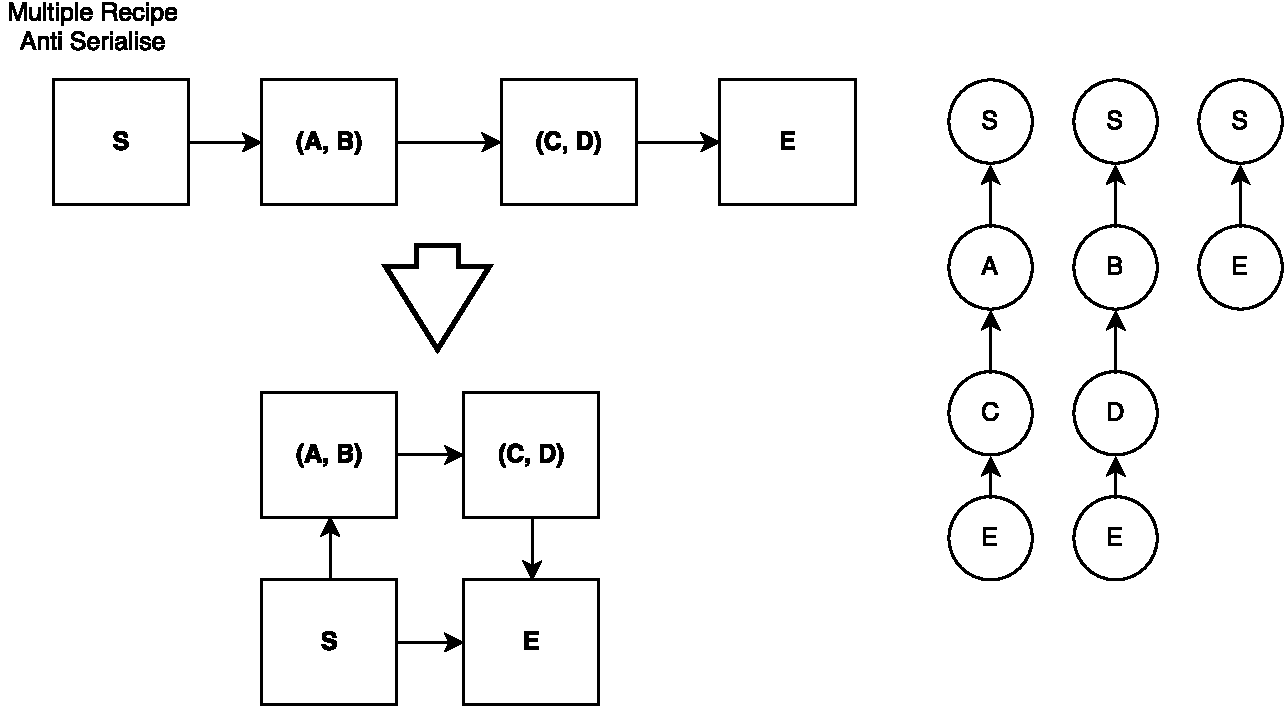
\includegraphics[width=1\textwidth]{figures/mras.pdf}
	\end{figure}
\end{frame}

\begin{frame}{Mere Robust Parallelize}
	\begin{itemize}
		\item Lige nu skal der være et 1 til 1 forhold mellem hvad de moduler vi gerne vil paralellisere kan og dem som vi bruger til at parallelisere med
		\item Vi gerne være i stand til at parallelisere en mængde af moduler så længe den mængde kan udføre det samme arbejde i den række den række følge, som den mængde vi parallelisere ud fra
	\end{itemize}
\end{frame}

\begin{frame} {Mere Robust Parallelize}
	\begin{figure}
		\centering
		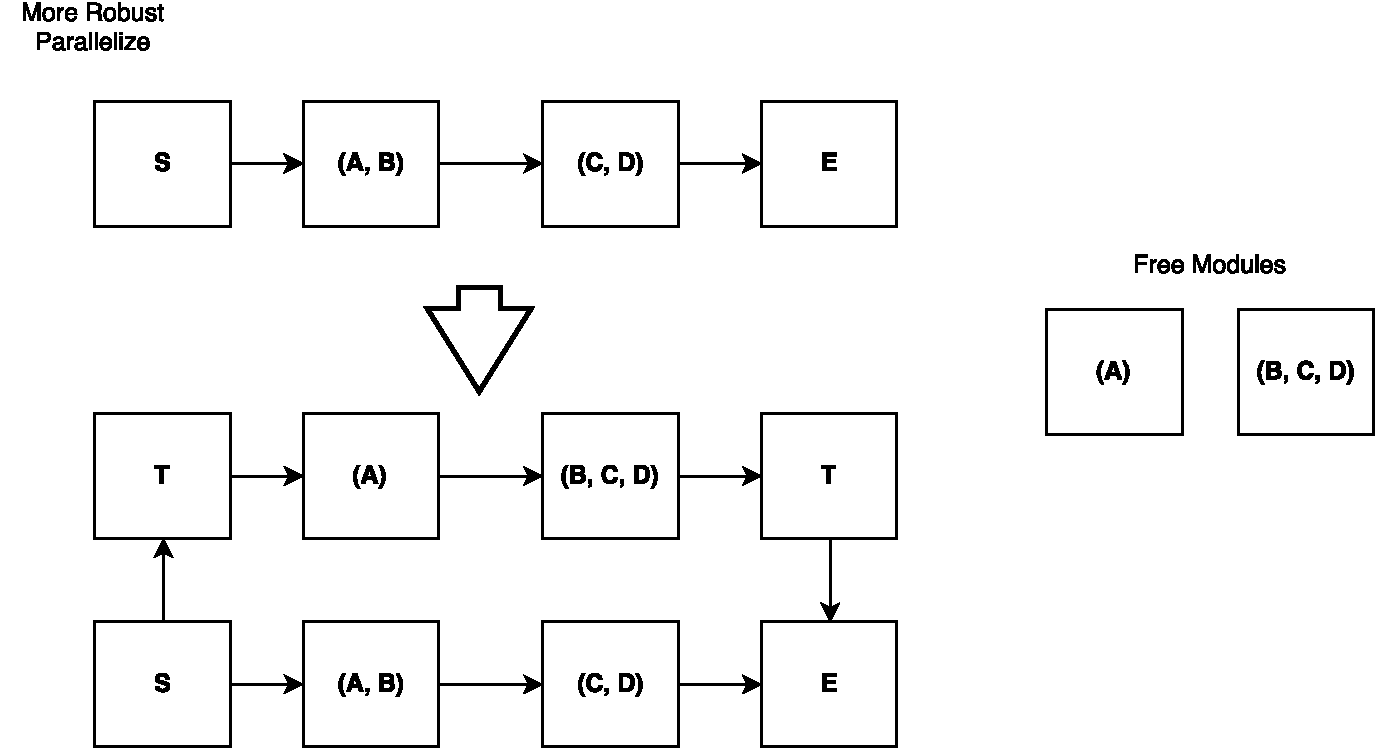
\includegraphics[width=1\textwidth]{figures/mrpara.pdf}
	\end{figure}
\end{frame}

\begin{frame}{Multiple Swap og Safe Swap}
	\begin{itemize}
		\item \textbf{Multiple Swap}: Igen være i stand til at swappe en mængde moduler ind eller ud, med en anden mængde moduler som er i stand til det samme arbejde i samme rækkefølge
		\item \textbf{Safe Swap}: Være i stand til at swappe moduler rundt i en konfiguration, hvor det stadigvæk er muligt at udføre recipes.
	\end{itemize}
\end{frame}



\section{Tabu Search}
\begin{frame} {Tabu Search}
	\begin{itemize}
		\item Tabu er en form for local search, men med hukommelse om hvad den tidliger har gjort.
		\item Hvorfor bruger vi Tabu Search?
		\item Hvorfor ikke en genetisk algorithme
	\end{itemize}
\end{frame}

\begin{frame} {Tabu Search}
	Hvordan fungere vores tabu search?
	\begin{itemize}
		\item Vi kan bruge vores transformations regler til at finde naboer
		\item Topologisk Sort af recipes til at finde $C_{naive}$
		\item Bruger langtidshukommelse til at gå tilbage til tidligere besøgte konfigurationer
		\item Bruger korttidshukommelse til at restriktere hvilke naboer vi må tage.
		\item Vi vælger at fase vores regler på forskellige tidspunkter for potentielt bedre søgninger
		\begin{itemize}
			\item Start: Mest sandsynelig at Anti-Serialisere
			\item Midt: Mest sandsynelig at Parallelisere
			\item Slut: Mest sandsynelig at Swappe
		\end{itemize}
	\end{itemize}
\end{frame}

\begin{frame}{Bedre Heuristikker til Tabu Search}
	\begin{itemize}
		\item Bedre håndtering af langtidshukommelse
		\begin{itemize}
			\item Bedre udvælgelse af hvornår noget skal i langtidshukommelse
			\item Måske ikke lade searchen tage en gammel route med det samme igen efter man er gået tilbage til et punkt i langtidshukommelsen.
		\end{itemize}
		\item Beskrive konfigurationer med flere attributer
		\begin{itemize}
			\item Beskriv sektioner i en konfiguration hvori ændrelser kan gøres til en tabu hvis de når et kriterie
		\end{itemize}
	\end{itemize}
\end{frame}

% Hvorfor Tabu Search
% Kobling til Regler 
% Andre Heuristiker vi kunne have brugt og forbedringer.

\section{Konklusion}
\begin{frame}{Konklusion}
	Så hvad har vi lavet?
	\begin{itemize}
		\item En UPPAAL model baseret på virkelige modulere fabrikker, som korrekt kan simulere dem
		\item Opsat regler for transformationer som kan har mulighed for at forbedre en konfiguration
		\item Implemeteret nævnte regler i en tabu search som er i stand til at søge efter en optimal konfiguration
	\end{itemize}
\end{frame}

\begin{frame}{Konklusion}
	\textit{How may we, given some order of items and set of available modules, be able to generate a factory configuration which has the fastest schedule of any other candidate configuration?}
	\begin{itemize}
		\item Løste vi vores problem?
	\end{itemize}
\end{frame}



% Kort om at vi løser problemet


{\aauwavesbg
\begin{frame}[plain,noframenumbering]
  \finalpage{Thank fordi i lyttede}
\end{frame}}
%%%%%%%%%%%%%%%%

\end{document}
